\chapter{Devices and Physical Limits}
\label{ch:devices}

\begin{chapterlead}
Non-Hermitian photonics is not only a theoretical framework---it is a
design language for optical devices. Exceptional-point sensors,
$\PT$-symmetric lasers, topological amplifiers, CPA switches, and
BIC-based cavities all exploit the physics developed in the preceding
chapters. The principal device concepts are surveyed, with operating
conditions derived from the Maxwell-level theory of Parts~I--III. The
chapter analyzes the physical limits imposed by noise, nonlinearity, and
fabrication disorder, and asks a question that the literature sometimes
avoids: which non-Hermitian advantages survive the constraints of
the real world? The organizing principle is that every device claim
must be tested against its noise floor, and every enhanced response must
be compared with its enhanced noise.
\end{chapterlead}


%% ================================================================
\section{$\PT$-symmetric lasers}
\label{sec:pt-lasers}

\subsection{Single-mode selection from mode non-orthogonality}
\label{ssec:pt-single-mode}

A conventional multimode laser oscillates in many longitudinal modes
simultaneously because the gain medium provides broadband amplification
without spectral discrimination. A $\PT$-symmetric laser, consisting of
a gain cavity coupled to a loss cavity of equal and opposite imaginary
refractive index, can enforce single-mode operation through a mechanism
rooted in the non-Hermitian spectral structure developed in
Chapter~\ref{ch:exceptional-points}.

Consider two coupled single-mode cavities with resonance frequencies
$\omega_0 \pm \delta/2$, coupling rate $\kappa$, and balanced gain/loss
$\pm g$. The effective Hamiltonian from Section~\ref{sec:ep2} is
\begin{equation}
 H_{\mathrm{eff}} = \begin{pmatrix}
 \omega_0 + \delta/2 + ig & \kappa \\
 \kappa & \omega_0 - \delta/2 - ig
 \end{pmatrix}.
 \label{eq:pt-laser-hamiltonian}
\end{equation}
Setting $\delta = 0$ for simplicity, the eigenfrequencies are
\begin{equation}
 \omega_\pm = \omega_0 \pm \sqrt{\kappa^2 - g^2}.
 \label{eq:pt-laser-eigenfreq}
\end{equation}
Below the EP ($g < \kappa$), both supermodes share the same imaginary
part---neither is preferentially amplified. Above the EP ($g > \kappa$),
one supermode acquires a net positive imaginary part while the other
acquires a net negative imaginary part; only the amplified mode reaches
the lasing threshold. This EP-mediated mode selection is intrinsically
non-Hermitian: it has no analogue in a Hermitian coupled-cavity system
where mode splitting is always real.

The physical mechanism extends to multimode cavities. If the system
supports $N$ longitudinal modes, each with its own detuning $\delta_m$,
the $\PT$ symmetry condition selects the mode whose gain--loss contrast
most efficiently exceeds the coupling threshold. Typically, this is the
mode closest to line center of the gain medium, where $g(\omega)$ is
largest. The remaining $N-1$ modes experience net loss and are
suppressed. This provides a mode-selection strategy based on
non-Hermitian spectral topology rather than on the conventional
mechanisms of gain competition, spatial hole burning, or intracavity
etalons.

\subsection{Experimental demonstrations}
\label{ssec:pt-laser-expt}

The first experimental demonstrations of $\PT$-symmetric single-mode
lasers were reported independently by two groups in 2014. Feng et al.\
fabricated coupled InGaAsP microring resonators with alternating
gain and loss regions, achieving single-mode lasing with a side-mode
suppression ratio (SMSR) exceeding $20\;\mathrm{dB}$; the conventional
counterpart (both rings pumped uniformly) exhibited multimode lasing.
Hodaei et al.\ demonstrated a similar concept using coupled microring
resonators with selective pumping and confirmed that the single-mode
selection persisted across a range of pump powers.

The key experimental signature is pump-dependent mode selection: at low
pump power the emission can be broad or multimode, while above the
non-Hermitian threshold one supermode acquires a clear gain advantage.
In an ideal two-mode model this transition is tied to the square-root
bifurcation near an EP (Section~\ref{sec:ep-topology}); in real lasers
gain saturation, spatial hole burning, and detuning smear the transition
and must be included before assigning an observed narrowing uniquely to
EP physics.

\subsection{Power, coherence, and the Petermann penalty}
\label{ssec:pt-laser-performance}

The output power and coherence of a $\PT$-symmetric laser are subject to
the same fundamental limits as any laser: the Schawlow--Townes linewidth
$\Delta\nu_{\mathrm{ST}}$, gain saturation, and spatial hole burning.
Near the EP, the Petermann excess noise factor
(Section~\ref{sec:petermann}) enhances the linewidth:
\begin{equation}
 \Delta\nu = K_{\mathrm{P}}\,\Delta\nu_{\mathrm{ST}},
 \qquad
 K_{\mathrm{P}} = \frac{|\langle\tilde{\EE}^{\mathrm{L}}|
 \tilde{\EE}^{\mathrm{L}}\rangle|\;
 |\langle\tilde{\EE}^{\mathrm{R}}|
 \tilde{\EE}^{\mathrm{R}}\rangle|}
 {|\langle\tilde{\EE}^{\mathrm{L}}|
 \tilde{\EE}^{\mathrm{R}}\rangle|^2},
 \label{eq:petermann-linewidth}
\end{equation}
where $K_{\mathrm{P}} \ge 1$ diverges as the EP is
approached~\cite{wang2020petermann}. Physically, the divergence arises
because the left and right eigenvectors become parallel at the EP, so
the biorthogonal projection $\langle\tilde{\EE}^{\mathrm{L}}|
\tilde{\EE}^{\mathrm{R}}\rangle \to 0$, and noise from the gain
reservoir is projected with increasing efficiency into the lasing mode.

For the two-mode dimer~\eqref{eq:pt-laser-hamiltonian} with $\delta=0$,
the Petermann factor can be computed explicitly. Defining the
non-orthogonality parameter $\theta$ through
$\cos\theta = g/\kappa$ in the $\PT$-symmetric phase,
\begin{equation}
 K_{\mathrm{P}} = \frac{1}{\sin^2\theta}
 = \frac{1}{1 - (g/\kappa)^2}.
 \label{eq:petermann-dimer}
\end{equation}
At the EP ($g = \kappa$), $K_{\mathrm{P}} \to \infty$. This expression
is written for the ideal unbroken-phase eigenvectors; in the broken
phase the Petermann factor must be evaluated from the actual above-threshold
linearized laser modes. The practical
design question for a $\PT$-symmetric laser is therefore whether
the single-mode purity gained by operating near the EP compensates for
the Petermann-enhanced linewidth. Typically, the optimal operating
point is somewhat above the EP, where the mode selectivity is strong
but $K_{\mathrm{P}}$ has not yet diverged catastrophically.

\paragraph{Example: microring $\PT$ laser dimer.}
Consider two coupled microring resonators at $\lambda = 1550\;\mathrm{nm}$
with $\Qfac_0 = 5 \times 10^4$, coupling rate
$\kappa = 2\pi \times 50\;\mathrm{GHz}$, and balanced gain/loss
$g = 1.2\kappa$ (broken $\PT$ phase).  The Schawlow--Townes linewidth
of a single ring is
$\Delta\nu_{\mathrm{ST}} \approx 30\;\mathrm{kHz}$.  In the broken
phase, both eigenfrequencies share the real part $\omega_0$, but their
imaginary parts split:
$\Im\omega_\pm = \pm\sqrt{g^2 - \kappa^2} = \pm 0.663\kappa
\approx \pm 2\pi \times 33\;\mathrm{GHz}$.
The amplified mode therefore has a net gain margin of
$\sim 33\;\mathrm{GHz}$ over the suppressed mode, providing robust
single-mode selection.  A representative Petermann factor of order
$K_{\mathrm{P}}\sim3$ would broaden the linewidth to
$\Delta\nu \sim 90$--$100\;\mathrm{kHz}$, illustrating that useful
mode-selection can coexist with a moderate noise penalty when the device
is not operated too close to the EP. The exact value requires the
above-threshold saturated modes, not only the passive two-mode dimer.

\subsection{Beyond single-mode: multi-element $\PT$ lasers}
\label{ssec:pt-multi}

The two-element dimer is the simplest $\PT$-symmetric laser, but the
concept extends to multi-element arrays. In a ring of $N$ coupled
cavities with alternating gain and loss, the non-Hermitian band
structure (Chapter~\ref{ch:complex-bands}) determines which modes lase.
The interplay between the $\PT$ phase transition and the band topology
can produce single-mode selection even in large arrays, provided that
the gain--loss contrast is tuned to the appropriate EP in the band
structure.

A particularly interesting configuration is the $\PT$-symmetric
laser array where the gain is concentrated at a topological edge state
(Section~\ref{ssec:nh-topo-laser}). This combines the $\PT$-mediated
mode selection with topological protection against backscattering,
potentially improving single-mode lasing robustness without relying only
on fine-tuned inter-cavity coupling.


%% ================================================================
\section{Exceptional-point sensors}
\label{sec:ep-sensors}

\subsection{Enhanced frequency splitting}
\label{ssec:ep-enhanced}

The square-root response at a second-order EP
(Section~\ref{sec:ep-sensing}) produces a frequency splitting
$\Delta\omega \propto \epsilon^{1/2}$ for a perturbation $\epsilon$,
which exceeds the linear splitting $\Delta\omega \propto \epsilon$ of a
conventional diabolic-point (DP) sensor for small $\epsilon$.

To make this concrete, consider a two-mode sensor with coupling
$\kappa$ tuned to the EP ($g = \kappa$). A small perturbation
$\epsilon$ (for example, the dielectric shift from a nanoparticle
binding to one of the cavities) splits the eigenfrequencies by
\begin{equation}
 \Delta\omega_{\mathrm{EP}} = 2\sqrt{\kappa\epsilon},
 \label{eq:ep-splitting}
\end{equation}
while the same perturbation applied to a DP sensor ($g = 0$, i.e.\ a
true degeneracy with orthogonal eigenvectors) lifts the degeneracy
linearly:
\begin{equation}
 \Delta\omega_{\mathrm{DP}} = 2\epsilon
 \label{eq:dp-splitting}
\end{equation}
when $\epsilon \ll \kappa$. The responsivity enhancement is therefore
\begin{equation}
 \frac{\Delta\omega_{\mathrm{EP}}}{\Delta\omega_{\mathrm{DP}}}
 = \frac{\sqrt{\kappa\epsilon}}{\epsilon}
 = \sqrt{\frac{\kappa}{\epsilon}},
 \label{eq:responsivity-enhancement}
\end{equation}
which diverges as $\epsilon \to 0$.

At an $n$th-order EP, the scaling is $\Delta\omega \propto
\epsilon^{1/n}$, promising even larger enhancements for higher-order
EPs. However, higher-order EPs require the simultaneous tuning of
$2(n-1)$ real parameters (Section~\ref{ssec:codimension}) and are
correspondingly more fragile.

\paragraph{Example: nanoparticle detection.}
A whispering-gallery-mode microsphere sensor operates at
$\lambda = 1550\;\mathrm{nm}$ with $\Qfac = 10^7$ and mode volume
$V_{\mathrm{eff}} \approx 300\;\mu\mathrm{m}^3$. A polystyrene
nanoparticle with radius $a = 8.5\;\mathrm{nm}$ and refractive index
$n_p = 1.59$ produces a perturbation
$\epsilon \approx (\omega_0/2)(n_p^2 - 1)\,a^3/V_{\mathrm{eff}}
\approx 2\pi \times 0.3\;\mathrm{MHz}$. With coupling
$\kappa = 2\pi \times 100\;\mathrm{MHz}$, the DP splitting is
$\Delta\omega_{\mathrm{DP}} \approx 2\pi \times 0.6\;\mathrm{MHz}$---well
below the linewidth $\gamma = \omega_0/(2\Qfac) \approx 2\pi \times
10\;\mathrm{MHz}$---while the EP splitting is
$\Delta\omega_{\mathrm{EP}} \approx 2\pi \times 11\;\mathrm{MHz}$,
comparable to the linewidth and therefore resolvable. The responsivity
enhancement is $\sqrt{\kappa/\epsilon} \approx 18$. As discussed
next, this enhanced splitting does not automatically translate into
enhanced detection precision.

\subsection{The noise problem: quantum Fisher information}
\label{ssec:noise-debate}

The fundamental question is whether the enhanced splitting translates
into enhanced signal-to-noise ratio (SNR). Near the EP, the
Petermann factor diverges, broadening the resonance linewidth by the
same factor that enhances the splitting.

Zhang et al.\ developed a quantum noise theory for EP sensors using
the quantum Langevin equations and input--output formalism~\cite{zhang2018quantum}.
Working in the two-mode bosonic framework, they computed the covariance
matrix of the output field and showed that the quantum Fisher
information (QFI) for estimating the perturbation $\epsilon$ satisfies
\begin{equation}
 \mathcal{F}_{\mathrm{EP}}(\epsilon) \le
 \mathcal{F}_{\mathrm{DP}}(\epsilon) \cdot f(\theta),
 \label{eq:qfi-bound}
\end{equation}
where $f(\theta) \to 1$ as $\theta \to 0$ (approaching the EP). The
Cram\'er--Rao bound then gives the minimum variance of any unbiased
estimator:
\begin{equation}
 \mathrm{Var}(\hat{\epsilon}) \ge \frac{1}{M\,\mathcal{F}(\epsilon)},
 \label{eq:cramer-rao}
\end{equation}
where $M$ is the number of measurements. In this steady-state linear
measurement model, with equal input power and integration time,
$\mathcal{F}_{\mathrm{EP}}\le\mathcal{F}_{\mathrm{DP}}$: the EP sensor
does not achieve a fundamental precision advantage over the corresponding
DP sensor. The enhanced splitting is accompanied by enhanced noise and
linewidth broadening.

The physical mechanism is transparent: the gain reservoir that creates
the EP also injects vacuum noise into the system. This noise is
amplified by the same non-orthogonal mode structure that amplifies the
signal, producing a noise floor that rises in lockstep with the
responsivity.

\begin{figure}[t]
 \centering
 
\includegraphics[width=0.95\linewidth]{fig_f18_ep_sensor_tradeoff.pdf}
 \caption{Exceptional-point sensing tradeoff in an idealized
 steady-state, equal-resource model. (a)~Near an EP, the responsivity
 scaling $\mathcal{R}\propto|\Delta p|^{-1/2}$ is accompanied by a
 Petermann-related noise scaling of the same order,
 $\sqrt{K}\propto|\Delta p|^{-1/2}$. The two curves are plotted with
 equal prefactors only to emphasize the shared asymptotic scaling.
 (b)~The corresponding SNR proxy
 $\mathcal{R}/\sqrt{K}$ is therefore approximately constant in this
 model. This illustrates why enhanced frequency splitting alone does
 not guarantee improved measurement precision; a real sensor must be
 judged by its complete noise budget and readout protocol~\cite{wang2020petermann,zhang2018quantum}.}
 \label{fig:ep-sensor-tradeoff}
\end{figure}


Wang et al.\ tested this tradeoff experimentally in a
Brillouin ring laser gyroscope operating near an EP. They measured the
Petermann-factor linewidth broadening and showed that the enhanced
Sagnac splitting was offset by enhanced noise, so that the measured
rotation sensitivity did not improve simply by operating at the
EP~\cite{wang2020petermann}.

\subsection{The noise problem: nonlinear and active systems}
\label{ssec:noise-nonlinear}

Zheng and Chong extended the analysis to nonlinear EP sensors---coupled
cavities operating above the lasing threshold---and showed that
nonlinearity does not rescue the SNR~\cite{zheng2024noise}. Their
analysis revealed three mechanisms by which noise degrades nonlinear
EP sensing:

\begin{enumerate}
 \item \textbf{Noise-induced EP shifting:} fluctuations in the
 intracavity intensity shift the saturated gain, moving the effective
 operating point away from the EP. The system never actually reaches
 the singular $\epsilon^{1/n}$ responsivity.
 \item \textbf{Order reduction:} the nonlinear steady state reduces
 the effective EP order, weakening the fractional-power enhancement.
 An EP$_2$ in the linear system may behave as an effective EP$_1$
 (no enhancement) in the saturated regime.
 \item \textbf{BdG fluctuation EPs:} the Bogoliubov--de~Gennes
 Hamiltonian governing small fluctuations around the nonlinear steady
 state has its own EP structure, which can produce noise divergences
 stronger than the Petermann estimate from the linear system.
\end{enumerate}

The conclusion is sobering: in the analyzed steady-state protocols,
neither linear nor nonlinear EP sensors achieve a fundamental SNR
advantage over DP sensors under the same resource constraints (same
cavity $\Qfac$, same input power, same integration time).

\subsection{When can EP sensing help?}
\label{ssec:ep-when}

Despite the noise-cancellation results, EP sensing may still offer
practical advantages in specific protocols:
\begin{enumerate}
 \item \textbf{Transient measurements:} reading a short-time ring-down
 can make the enhanced dynamical response easier to observe in a fixed
 bandwidth. The relevant figure of merit is the full transient estimator
 variance, not only the steady-state linewidth.
 \item \textbf{Interferometric readout:} heterodyne or self-heterodyne
 schemes that measure the beat frequency between the two split
 modes may reject technical common-mode noise, even though they do not
 remove the fundamental quantum-noise accounting.
 \item \textbf{Active feedback:} real-time feedback can stabilize
 technical drift of the operating point near the EP. It improves
 practical stability but adds its own measurement noise and control
 bandwidth limits.
 \item \textbf{Exceptional surfaces:} in parameter spaces where EPs
 form codimension-one surfaces rather than isolated points,
 the system can be operated on the exceptional surface without
 fine-tuning, potentially reducing the sensitivity to drift.
\end{enumerate}
The general lesson is that the \emph{responsivity} of an EP sensor is
genuinely enhanced, but converting that responsivity into enhanced
\emph{precision} requires a measurement protocol whose complete noise
budget is better than the reference sensor. The distinction between responsivity and
precision is a recurrent theme in non-Hermitian device physics and
should be kept in mind whenever an ``enhanced sensitivity'' claim is
evaluated.


%% ================================================================
\section{BIC-based lasers and cavities}
\label{sec:bic-devices}

\subsection{From radiation suppression to lasing threshold}
\label{ssec:bic-laser-device}

Bound states in the continuum (Chapter~\ref{ch:bic-topology}) provide a
fundamentally different route to high-$\Qfac$ lasing. A photonic
crystal slab laser operating near a BIC exploits the topological
suppression of radiation loss to achieve single-mode lasing with high
power and narrow linewidth, without requiring a physical mirror or
cavity boundary.

The lasing condition connects the BIC physics to the Maxwell-level
framework of this book. The radiation quality factor near a BIC scales
as (Section~\ref{ssec:finite-size})
\begin{equation}
 \Qfac_{\mathrm{rad}}(k) \propto \frac{1}{|c(k)|^2},
 \label{eq:bic-q-rad}
\end{equation}
where $c(k)$ is the radiation amplitude introduced in
Section~\ref{ssec:radiation-amplitude}. At a BIC, $c(k_{\mathrm{BIC}}) = 0$
and $\Qfac_{\mathrm{rad}} \to \infty$. Adding gain to the slab
reduces the total quality factor to
\begin{equation}
 \frac{1}{\Qfac_{\mathrm{tot}}} = \frac{1}{\Qfac_{\mathrm{rad}}}
 + \frac{1}{\Qfac_{\mathrm{abs}}} - \frac{1}{\Qfac_{\mathrm{gain}}},
 \label{eq:bic-total-q}
\end{equation}
where $\Qfac_{\mathrm{abs}}$ accounts for material absorption and
$\Qfac_{\mathrm{gain}}$ accounts for optical gain. The lasing threshold
is reached when $\Qfac_{\mathrm{tot}} \to \infty$, i.e.,
\begin{equation}
 \frac{1}{\Qfac_{\mathrm{gain}}} = \frac{1}{\Qfac_{\mathrm{rad}}}
 + \frac{1}{\Qfac_{\mathrm{abs}}}.
 \label{eq:bic-threshold}
\end{equation}
Near the BIC, $\Qfac_{\mathrm{rad}}$ is very large, so the threshold is
determined primarily by material absorption: the BIC suppresses the
radiation channel, leaving only the material loss as the dominant
threshold-setting mechanism. In finite active devices the threshold is
also limited by finite aperture, pump overlap, nonradiative recombination,
and thermal rollover, but radiation suppression is the central reason for
the low thresholds observed in BIC lasers.

The finite-size limitation is set by the momentum spread
$\Delta k \sim 1/N$ of a cavity with $N$ periods. For an isolated
charge-one BIC, $\Qfac_{\mathrm{finite}} \propto N^2$, which can be
modest for small cavities.

\subsection{Super-BIC lasers}
\label{ssec:super-bic-device}

The topological charge-merging strategy of Section~\ref{sec:bic-merging}
can improve the finite-size scaling. When symmetry and
charge conservation force the lower-order radiation amplitudes to cancel
at the merged point, the radiation amplitude vanishes to higher order:
\begin{equation}
 c(k) \propto k^{|q|} \quad \Longrightarrow \quad
 \Qfac_{\mathrm{finite}} \propto N^{2|q|}.
 \label{eq:super-bic-scaling}
\end{equation}
For the super-BIC design discussed in Chapter~\ref{ch:bic-topology}, the
leading radiation rate scales as $k^6$, so the finite-size $\Qfac$ can
scale as $N^6$, compared with the $N^2$ scaling of an
isolated BIC. This scaling is not guaranteed by charge addition alone;
it also relies on the symmetry of the merged configuration.

Hwang et al.\ demonstrated a super-BIC laser in an InGaAsP photonic
crystal slab with a square lattice of air holes~\cite{hwang2021ultralow}.
By tuning the lattice constant to the merging point
($a \approx \SI{576.3}{nm}$), they achieved:
\begin{itemize}
 \item Radiation loss scaling of $k^6$ instead of $k^2$.
 \item Measured threshold of $\sim\SI{1.47}{kW/cm^2}$---roughly
 $50$ to $10^7$ times lower than previous BIC nanolasers.
 \item Quality factor up to $\sim 7300$ in a cavity of only
 $15 \times 15$ periods.
 \item A strongly confined far-field image consistent with the $k^6$
 angular suppression.
\end{itemize}
The super-BIC concept demonstrates that topological charge engineering
can convert a fundamental limitation (the finite-size $\Qfac$ penalty)
into a practical design advantage.

\subsection{BZF-BIC cavities}
\label{ssec:bzf-device}

Brillouin-zone-folding BICs (Section~\ref{sec:bzf-bic}) offer a
complementary approach: instead of steepening the $\Qfac$ scaling at a
single $k$-point, they sustain high $\Qfac$ over a broad momentum
range. Wang et al.\ showed that BZF-BICs retain $\Qfac$ at least ten
times higher than conventional BICs under the same structural
disorder~\cite{wang2023brillouin}, making them attractive for large-area
lasing and sensing applications where momentum-space averaging is
important.

\subsection{Quasi-BIC applications beyond lasing}
\label{ssec:quasi-bic-apps}

Away from the exact BIC condition, the system supports a quasi-BIC
resonance with finite but very large $\Qfac$. The quasi-BIC produces
a sharp Fano line shape in the scattering spectrum
(Section~\ref{ssec:quasi-bic-resonances}), which is useful for applications beyond
lasing:
\begin{itemize}
 \item \textbf{Refractive-index sensing:} the figure of merit
 $\mathrm{FOM}=S/\delta\lambda
 = \Delta\lambda/(\Delta n\,\delta\lambda)$,
 where $S=\Delta\lambda/\Delta n$ is the sensitivity,
 $\delta\lambda$ is the linewidth, and $\Delta n$ is the index change, benefits
 directly from the high $\Qfac$ of the quasi-BIC. Reported FOMs
 for quasi-BIC metasurfaces exceed $10^3$ in the near-infrared.
 \item \textbf{Nonlinear enhancement:} resonant field buildup can
 strongly enhance nonlinear conversion, with the precise power of
 $\Qfac$ depending on whether the pump, signal, and generated frequency
 are all resonant and critically coupled. This makes quasi-BIC
 resonances attractive platforms for nonlinear nanophotonics, but the
 scaling is device- and process-dependent.
 \item \textbf{Spectral filtering:} the asymmetric Fano profile of a
 quasi-BIC can be engineered to produce narrow-band filters with
 tunable center wavelength and bandwidth by adjusting the structural
 perturbation that breaks the BIC condition.
\end{itemize}


%% ================================================================
\section{Coherent perfect absorbers and switches}
\label{sec:cpa-devices}

\subsection{CPA as a scattering zero}
\label{ssec:cpa-switch}

A coherent perfect absorber (Section~\ref{ssec:zeros}) operates at a zero
of the scattering matrix: with the correct phase and amplitude
relationship between two input beams, all light is absorbed. From the
pole-zero framework of Chapter~\ref{ch:poles-zeros}, the CPA condition
corresponds to a real-frequency zero of $\det S(\omega)$.

The CPA device functions as an all-optical switch: modulating the
relative phase $\phi$ between the two input beams sweeps the system
between perfect absorption ($\phi = \phi_0$) and near-total
transmission ($\phi = \phi_0 + \pi$). The switching contrast is
\begin{equation}
 \mathcal{C} = \frac{T_{\max}}{T_{\min}}
 = \frac{(1 + |r|)^2}{(1 - |r|)^2},
 \label{eq:cpa-contrast}
\end{equation}
where $|r|$ is the single-channel reflection coefficient at the CPA
frequency. For $|r| \to 1$ (high-finesse cavity), the contrast diverges,
but in practice it is limited by absorption losses and fabrication
imperfections.

The switching speed is set by the cavity lifetime
$\tau = \Qfac/\omega_0$; for a $\Qfac \sim 10^3$ resonator at
$\lambda = 1550\;\mathrm{nm}$, $\tau \approx 0.8\;\mathrm{ps}$---faster
than electronic switches by orders of magnitude.

\begin{figure}[t]
 \centering
 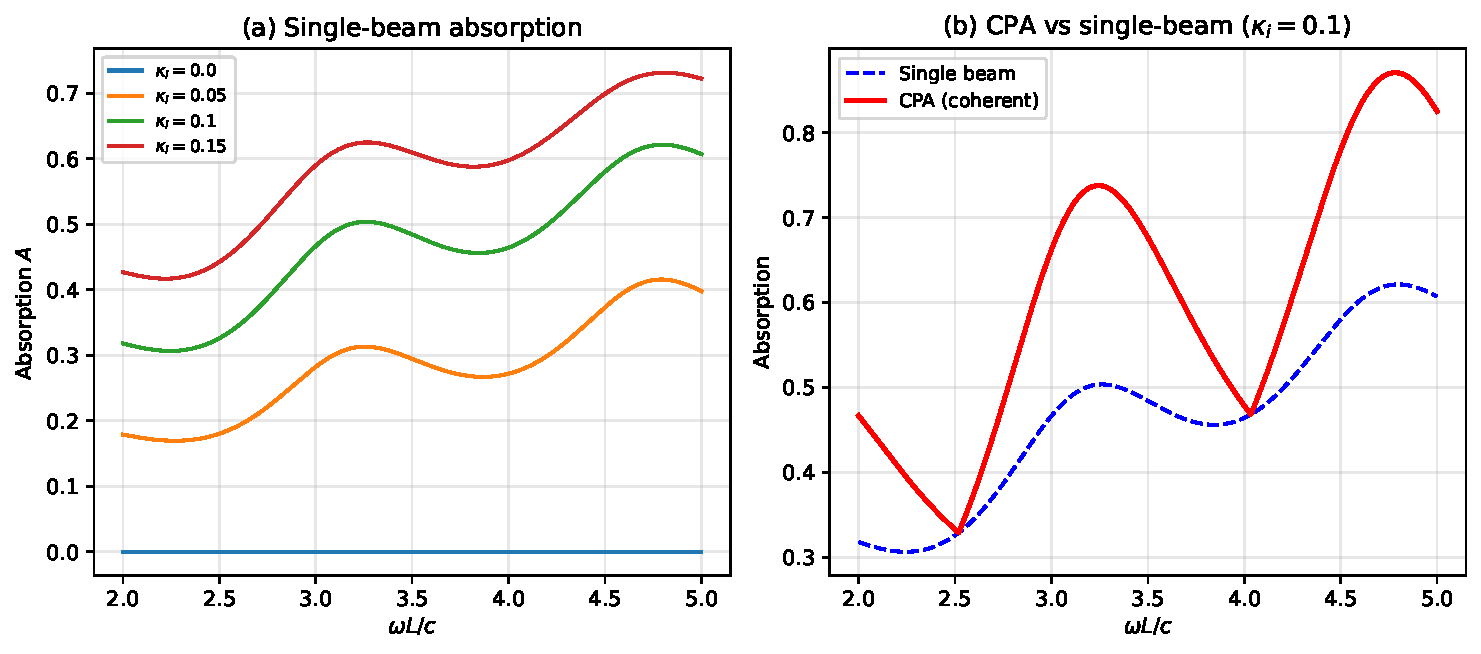
\includegraphics[width=0.85\linewidth]{figures/fig_f18_cpa_switching.pdf}
 \caption{Coherent perfect absorption in a lossy Fabry--P\'erot cavity
 ($n = 2$).
 (a)~Single-beam absorption for different extinction coefficients
 $\kappa_i$: increasing material loss raises the peak absorption but
 broadens the resonance.
 (b)~Comparison of single-beam (dashed) and coherent two-beam (solid)
 absorption for $\kappa_i = 0.1$. Under coherent illumination the
 absorption reaches near-unity at the CPA frequency, demonstrating the
 interferometric enhancement that is the hallmark of CPA---the
 time-reversed counterpart of lasing
 (Section~\ref{sec:time-reversal}).}
 \label{fig:cpa-switching}
\end{figure}

\subsection{CPA-laser devices}
\label{ssec:cpa-laser-device}

At the CPA-laser point (Chapter~\ref{ch:poles-zeros}), the same device
simultaneously acts as a laser (for one input configuration) and a
perfect absorber (for the conjugate configuration). From the scattering
matrix formalism, this corresponds to
\begin{equation}
 \det S(\omega_{\mathrm{CPA\text{-}laser}}) = 0
 \quad \text{and} \quad
 \det S(\omega_{\mathrm{CPA\text{-}laser}}) \text{ has a pole},
 \label{eq:cpa-laser-condition}
\end{equation}
i.e., a simultaneous pole and zero at the same real frequency. In a
$\PT$-symmetric system, the symmetry constrains poles and zeros to occur
in conjugate pairs (Section~\ref{sec:pt-scattering}), making the
CPA-laser condition possible when a pole and its time-reversed zero meet
on the real axis. The symmetry is a constraint, not by itself a guarantee
that a real-frequency pole-zero coincidence occurs without tuning.

The dual CPA-laser functionality enables phase-controlled routing: by
tuning the input phase, the device can be switched between amplification
and absorption, with the transition controlled by the pole-zero
structure of the scattering matrix.

The practical challenge is maintaining the precise gain--loss balance
required by the CPA-laser condition. Any imbalance shifts the pole
and zero apart, reducing the contrast. The critical distinction,
emphasized in Section~\ref{ssec:cpa-vs-ep}, is that the CPA-laser
condition depends on fine-tuned scattering singularities, not on
topological invariants. Topological protection (from BIC charges or
Chern edge states) does \emph{not} protect the CPA-laser point, because
a topological invariant constrains the \emph{number} of singularities in
a region of parameter space, not their \emph{positions}.

\subsection{Practical CPA limitations}
\label{ssec:cpa-limits}

Several practical constraints limit CPA device performance:
\begin{itemize}
 \item \textbf{Beam alignment:} perfect absorption requires precise
 control of the phase, amplitude, and spatial mode of two input
 beams. Any mismatch reduces the absorption efficiency.
 \item \textbf{Bandwidth:} the CPA condition is satisfied at a single
 frequency; broadband operation requires a resonator design with
 overlapping or broadened zeros.
 \item \textbf{Nonlinear effects:} at high input powers, the CPA
 condition shifts due to Kerr and thermal nonlinearities, limiting
 the useful power range.
\end{itemize}


%% ================================================================
\section{Topological lasers}
\label{sec:topo-lasers}

\subsection{Topological insulator lasers}
\label{ssec:topo-laser}

A topological insulator laser~\cite{bandres2018topological,harari2018topological} combines a photonic topological insulator
(Chapter~\ref{ch:berry-maxwell}) with optical gain. The lasing mode
propagates along the topological edge channel, where elastic
backscattering from fabrication defects is strongly suppressed as long as the
topological gap and the protecting symmetries are maintained. The result
can be a laser with robust single-mode operation and high slope
efficiency, but gain competition, disorder-induced loss, and finite-size
coupling still matter.

Several platforms have demonstrated topological lasing:
\begin{itemize}
 \item \textbf{Microring arrays:} coupled microring resonators with
 alternating link-ring couplers that implement a photonic
 anomalous quantum Hall lattice. Bandres et al.\ (2018)
 demonstrated edge-mode lasing with a slope efficiency comparable
 to conventional ring lasers but with improved
 robustness against intentional defects---removing a ring from the
 edge path did not suppress lasing, whereas removing a bulk-mode
 ring had no effect.
 \item \textbf{Valley-Hall photonic crystals:} triangular-hole
 photonic crystal slabs with broken inversion symmetry, supporting
 valley-polarized edge states. Lasing along the domain wall was
 shown to be robust against sharp $120^\circ$ bends, with
 threshold comparable to the straight-edge case.
 \item \textbf{SSH micropillar chains:} one-dimensional arrays of
 semiconductor micropillars with alternating coupling, where
 topological edge modes lase selectively at the chain boundary.
 The topological gap protects the edge state from hybridizing
 with bulk modes, providing a natural single-mode filter.
\end{itemize}

The key metric for a topological laser is not the absolute threshold or
slope efficiency---these are comparable to conventional lasers---but
rather the \emph{robustness} of the single-mode operation and the
\emph{insensitivity} to disorder.

\subsection{Non-Hermitian topological lasers}
\label{ssec:nh-topo-laser}

Adding non-Hermitian ingredients (gain/loss patterning, $\PT$ symmetry)
to topological structures creates a richer design space. For example,
selectively pumping only the edge region of a topological lattice can
enforce single-mode topological lasing without requiring uniform gain
across the entire structure---reducing the power budget and avoiding
multimode instabilities from bulk gain.

This strategy exploits non-Hermitian gain selectivity rather than the
skin effect by itself: patterning the imaginary part of the on-site
potential to provide gain only near the boundary preferentially amplifies
edge modes and suppresses bulk modes. If the underlying lattice also has
point-gap winding, true skin accumulation can further reshape the modal
profiles, but boundary pumping alone should not be identified with the
NHSE.

An important distinction is between \emph{topological protection of
the lasing mode} and \emph{topological origin of the lasing
threshold}. In most topological lasers~\cite{ota2020active,zhu2026topology,al2024topological}, the topology protects the
spatial profile of the lasing mode (preventing backscattering and
maintaining single-mode character), but the threshold itself is set by
the gain--loss balance, which is not topologically protected.

\subsection{Non-Hermitian skin amplifiers}
\label{ssec:skin-amplifier}

The standard non-Hermitian skin effect localizes an extensive set of
right eigenstates at one boundary
(Chapter~\ref{ch:skin-effect}). In a system with gain, this
localization produces exponential amplification of signals injected at
the opposite boundary, as they propagate toward the skin-effect edge.
Using the Hatano--Nelson model of Section~\ref{sec:hatano-nelson}, the
ideal amplitude factor grows exponentially with system size:
\begin{equation}
 G = \left(\frac{t_R}{t_L}\right)^L,
 \label{eq:skin-gain}
\end{equation}
where $t_R/t_L$ is the hopping asymmetry ratio and $L$ is the number of
unit cells. If $G$ is interpreted as a power gain, the corresponding dB
value is $10\log_{10}G$; if it is a field-amplitude factor, the power
gain scales as $|G|^2$. For $t_R/t_L=2$ and $L=20$, the ideal amplitude
factor is $2^{20}\approx10^6$, corresponding to an enormous small-signal
power gain before saturation and noise are included.

The direction of accumulation is tied to the sign of the point-gap
winding of the PBC spectrum around the reference energy
(Section~\ref{sec:winding}). This provides a route to directional
amplification without necessarily using magneto-optical materials,
although a physical photonic implementation must still realize effective
asymmetric hopping and control added noise.

The practical challenge is implementing the required asymmetric hopping
in a photonic platform. Photonic mesh lattices with fiber loops of
different lengths, time-modulated coupled resonators, and
magnetically biased photonic crystals have been proposed as physical
realizations.


%% ================================================================
\section{Active non-Hermitian metasurfaces}
\label{sec:nh-metasurfaces}

\subsection{Wavefront control with gain and loss}
\label{ssec:nh-wavefront}

Non-Hermitian metasurfaces~\cite{cui2024roadmap,ma2022information} extend the wavefront-control capabilities of
passive metasurfaces by incorporating gain and loss as additional design
degrees of freedom. In a passive metasurface, each meta-atom controls
the phase and amplitude of the transmitted or reflected field through
its geometric and material parameters. In a non-Hermitian metasurface,
each meta-atom additionally carries a complex refractive index with a
controllable imaginary part, enabling independent control of the phase,
amplitude, and gain/loss profile across the surface.

From the scattering-matrix perspective (Chapter~\ref{ch:poles-zeros}),
each meta-atom is characterized by its complex transmission and
reflection coefficients. By engineering the pole-zero structure of each
meta-atom, the metasurface can implement arbitrary complex transfer
functions, achieving functionalities impossible with purely passive
elements---for example, asymmetric reflection profiles where the
reflected wavefront depends on the illumination direction.

\subsection{$\PT$-symmetric metasurfaces}
\label{ssec:pt-metasurface}

A metasurface with a $\PT$-symmetric gain/loss distribution can exhibit
unidirectional properties analogous to those of $\PT$-symmetric Bragg
gratings (Section~\ref{ssec:unidirectional}). At the $\PT$-breaking
point, the metasurface can be invisible from one side while reflecting
from the other, creating a flat-optics analogue of unidirectional
invisibility.

\subsection{CPA metasurfaces}
\label{ssec:cpa-metasurface}

A metasurface designed to operate at the CPA condition provides a
thin-film all-optical modulator. By controlling the relative phase
of two counter-propagating beams incident on the metasurface, the
absorption can be switched from near-zero to near-unity, enabling
modulation at sub-picosecond timescales with a device footprint of
a single wavelength.


%% ================================================================
\section{Physical limits}
\label{sec:physical-limits}

Every non-Hermitian device advantage comes with a physical cost. This
section catalogs the principal limits in a unified framework and
provides quantitative estimates that allow device designs to be compared
on an equal footing.

\subsection{Quantum noise and the Petermann factor}
\label{ssec:quantum-noise}

All non-Hermitian photonic devices are ultimately limited by quantum
noise. The fluctuation-dissipation theorem requires that any system with
loss also has noise; gain media amplify both signal and spontaneous
emission. Near an EP, the enhanced Petermann
factor~\eqref{eq:petermann-linewidth} amplifies the noise, setting a
fundamental floor on the sensitivity of EP-based devices.

The Petermann factor reflects the non-orthogonality of the modes in the
biorthogonal expansion of Chapter~\ref{ch:qnm}. In a system with
$K_{\mathrm{P}} = 100$ (easily achieved within
$|\Delta p|/\kappa \sim 0.1$ of a second-order EP), the spontaneous
emission rate into the lasing mode is enhanced by a factor of 100
relative to the Hermitian limit, degrading the laser coherence and the
sensor precision by the same factor.

For an $n$th-order EP, the Petermann factor diverges as
(Section~\ref{ssec:petermann-ep})
\begin{equation}
 K_{\mathrm{P}} \propto \frac{1}{|\Delta p|^{2(n-1)}},
 \label{eq:petermann-scaling-device}
\end{equation}
where $\Delta p$ is the distance from the EP in parameter space. The
noise penalty therefore grows faster with EP order than the responsivity
enhancement ($\epsilon^{1/n}$), and the net SNR actually \emph{decreases}
with increasing EP order for fixed resource constraints.

\subsection{Gain saturation and nonlinearity}
\label{ssec:nonlinearity-limits}

The linear non-Hermitian framework of this book is valid below or near
the lasing threshold. Above threshold, gain saturation introduces
nonlinear corrections that stabilize the system (preventing runaway
amplification) but also modify the EP structure and the topological
invariants.

The gain saturation model of Section~\ref{sec:gain-media} gives
\begin{equation}
 g(I) = \frac{g_0}{1 + I/I_{\mathrm{sat}}},
 \label{eq:gain-saturation-device}
\end{equation}
where $g_0$ is the small-signal gain, $I$ is the intracavity intensity,
and $I_{\mathrm{sat}}$ is the saturation intensity. For EP sensors
operating above threshold, the nonlinear steady state shifts the
operating point away from the EP by an amount
\begin{equation}
 \delta g \sim g_0 \frac{I_{\mathrm{ss}}}{I_{\mathrm{sat}}},
 \label{eq:ep-shift-nonlinear}
\end{equation}
where $I_{\mathrm{ss}}$ is the steady-state intracavity intensity. This
shift effectively reduces the EP order and weakens the $\epsilon^{1/n}$
responsivity~\cite{zheng2024noise}.

For topological invariants, gain saturation can change the sign of the
imaginary part of the permittivity, potentially opening or closing
point gaps and modifying the winding numbers. The interplay between
nonlinearity and non-Hermitian topology is an active research frontier
(Chapter~\ref{ch:open-problems}).

\subsection{Fabrication disorder}
\label{ssec:disorder}

Real photonic devices have fabrication imperfections that perturb the
$\PT$ symmetry condition, shift EPs, and break the gain--loss balance.
Different non-Hermitian features have different robustness:
\begin{itemize}
 \item \textbf{Topologically constrained:} BIC far-field charges
 (Section~\ref{sec:bic-charge}), Chern edge states, and
 point-gap/skin-effect orientation are robust to perturbations that
 preserve the relevant gap, symmetry, and radiation-channel structure.
 They change only when the corresponding topological description breaks
 down or a topological transition occurs.
 \item \textbf{Fine-tuned:} the precise EP location, the CPA-laser
 condition, the $\PT$ symmetry balance, and the gain--loss
 threshold all depend on continuous parameters and are shifted
 by any fabrication error.
\end{itemize}
The practical design challenge is to maximize the fraction of the device
functionality that relies on topological protection, while accepting
that fine-tuned parameters will need active stabilization or tolerance
engineering.

A useful figure of merit for disorder robustness is the \emph{topological
gap ratio}---the ratio of the topological gap $\Delta_{\mathrm{top}}$
to the typical disorder-induced level broadening $\Gamma_{\mathrm{dis}}$.
When $\Delta_{\mathrm{top}}/\Gamma_{\mathrm{dis}} \gg 1$, topologically
protected features survive; when $\Delta_{\mathrm{top}}/\Gamma_{\mathrm{dis}}
\lesssim 1$, the topological protection breaks down and device
performance reverts to the non-topological baseline.

\subsection{Thermal and power limits}
\label{ssec:thermal}

Gain media dissipate heat. In semiconductor lasers, the thermal load
from the pump current limits the maximum gain that can be applied before
thermal rollover degrades the performance. $\PT$-symmetric devices,
which require a precise balance between gain and loss, are particularly
sensitive to thermal drifts because the gain medium and the loss medium
have different thermal coefficients.

For BIC-based devices, the ultra-high $\Qfac$ near the BIC reduces the
threshold power, mitigating the thermal problem. The super-BIC laser of
Hwang et al.\ achieved a threshold of $\sim\SI{1.47}{kW/cm^2}$---orders
of magnitude below conventional nanolasers---precisely because the
topological charge merging minimized the radiation
loss~\cite{hwang2021ultralow}.

\subsection{Gain--bandwidth constraints}
\label{ssec:gain-bandwidth}

A fundamental constraint on non-Hermitian devices comes from the
gain--bandwidth product. The Kramers--Kronig relations
(Section~\ref{sec:kramers-kronig}) link the real and imaginary parts
of the permittivity, so gain over a finite bandwidth implies a
corresponding frequency-dependent phase shift. For a Lorentzian gain
medium with peak gain $g_0$ and gain bandwidth $\Delta\omega_g$, the
gain--bandwidth product is
\begin{equation}
 g_0 \cdot \Delta\omega_g = \frac{N_{\mathrm{inv}}\,\sigma_0\,c}{n_g},
 \label{eq:gain-bandwidth}
\end{equation}
where $N_{\mathrm{inv}}$ is the population inversion density,
$\sigma_0$ is the stimulated emission cross-section, and $n_g$ is the
group index. This places an upper bound on the gain that can be
achieved over a given bandwidth, limiting the number of modes that can
be simultaneously pushed above threshold in a $\PT$-symmetric laser
and constraining the operational bandwidth of EP sensors.

\subsection{Summary: device concepts and their physical limits}
\label{ssec:device-summary}

\begin{figure}[t]
 \centering
 
\includegraphics[width=0.95\linewidth]{fig_f18_device_comparison.pdf}
 \caption{Quantitative comparison of five non-Hermitian photonic device
 classes discussed in this chapter.
 (a)~Representative quality factor $\Qfac$ on a logarithmic scale.
 The EP sensor achieves the highest $\Qfac \sim 10^6$ through
 whispering-gallery modes, while the CPA absorber operates at a
 modest $\Qfac \sim 2 \times 10^3$ because critical coupling demands
 matched radiative and absorptive rates.
 (b)~Lasing threshold in kW\,cm$^{-2}$ for laser-type devices; the
 EP sensor and CPA absorber are passive and marked N/A. The
 super-BIC laser has the lowest threshold
 ($1.47\;\mathrm{kW\,cm}^{-2}$) thanks to the $k^6$
 radiation-loss suppression of merged BICs. Data are representative
 values from the literature discussed in the text.}
 \label{fig:device-comparison}
\end{figure}

Table~\ref{tab:device-limits} summarizes the principal non-Hermitian
device concepts, their key operating mechanisms, the source of
their non-Hermitian advantage, and the physical limit that constrains
their performance.

\begin{table}[t]
\centering
\small
\caption{Non-Hermitian photonic device concepts and their physical limits.}
\label{tab:device-limits}
\begin{tabular}{@{}p{3.0cm}p{3.2cm}p{3.2cm}p{3.8cm}@{}}
\toprule
\textbf{Device} & \textbf{Mechanism} & \textbf{NH advantage} & \textbf{Primary limit} \\
\midrule
$\PT$ laser & EP mode selection & Single-mode purity & Petermann noise, thermal drift \\
EP sensor & $\epsilon^{1/n}$ splitting & Enhanced responsivity & Petermann noise cancels SNR gain \\
BIC laser & Topological $\Qfac$ & Ultralow threshold & Finite-size $\Qfac$, disorder \\
Super-BIC laser & Charge merging & Steeper finite-size $\Qfac$ scaling & Lattice-constant tolerance \\
CPA switch & Scattering zero & All-optical modulation & Beam alignment, bandwidth \\
CPA-laser & Pole-zero coincidence & Dual amplification/absorption & Fine-tuned gain--loss balance \\
Topological laser & Edge-state lasing & Disorder robustness & Threshold not topologically protected \\
Skin amplifier & NHSE localization & Directional small-signal gain & Asymmetric hopping, saturation, noise \\
\bottomrule
\end{tabular}
\end{table}

\begin{takeaway}[Promise and limits of non-Hermitian devices]
Non-Hermitian photonic devices exploit exceptional points, $\PT$
symmetry, CPA-laser duality, BIC topology, and the skin effect to
achieve functionalities impossible in Hermitian systems: single-mode
lasing, enhanced sensing responsivity, all-optical switching, and
directional amplification. But every advantage comes with a physical
cost---the Petermann noise penalty, gain saturation, fabrication
sensitivity, or thermal load---that must be assessed quantitatively
against the specific application. The most robust devices are those
that anchor their functionality in topological invariants rather than
fine-tuned parameters, and the most honest assessments compare not just
the enhanced response but the enhanced response \emph{together with}
the enhanced noise.
\end{takeaway}
